\documentclass{article}
\usepackage[utf8]{inputenc}
\usepackage[brazil]{babel}
\usepackage{hyperref}
\usepackage[paper=a4paper,lmargin=1.5cm, rmargin=1.5cm, tmargin=1.6cm, bmargin=1.5cm]{geometry}
\usepackage{graphicx}

\title{\textit{ALGORITMOS E ESTRUTURAS DE DADOS III} - Anotações de aula}
\author{fpk07@c3sl.ufpr.br}
\date{15/12/2010}


\begin{document}


\maketitle

\tableofcontents

\section{Introdução}

Essa apostila tem como finalidade ajudar os alunos de ALG III do curso B.C.C. da
UFPR. Os capítulos não seguirão o fluxo das aulas ministradas em ALG III,
contudo abrangerão todos os temas cobrados em prova e dados em aula. Essa
apostila foi baseada nas aulas da turma 2010-2-B.\\
Essa apostila tem ênfase em dar dicas de estudo e comenta dicas importantes para
bom andamento do estudo; A maior parte do conteúdo será referenciado em
apostilas e applets.

\begin{quotation}
\textit{IMPORTANTE:} O autor não se responsabiliza por nenhuma questão respondida
erroneamente ou informação errada. A apostila sempre estará aberta a sugestões e modificações. É
responsabilidade do leitor verificar TODAS as respostas em bons livros,
principalmente nos das referências de estudo que os professores passam.
Wikipedia e sites semelhantes, embora contenham boa fonte de conteúdo com
qualidade, não podem ser usados no meio acadêmico como qualquer tipo de
referência.
\end{quotation}

\section{Árvores}
Algumas definições importantes:

\begin{itemize}
	\item Pai: Um nó que possui descendentes (filhos);
	\item Filho: Descendentes de alguém bem óbvio; :)
	\item Avô/tio: óbvios;
	\item Nós: São os nós que podem ou não conter as chaves (dados);
	\item Raíz: Nó extremo superior da árvore;
	\item Folhas: extremos inferiores da árvore;
	\item Nível: Começa em 0 (zero) na raíz;
	\item Altura: Nível máximo;
\end{itemize}

\section{Árvores binárias de Busca}
Cada pai possui dois filhos, o esquerdo e o direito.

\subsection{Links de referência para estudo}
\begin{itemize}
	\item \href{http://equipe.nce.ufrj.br/adriano/c/apostila/arvore.htm}{Árvores binárias}
	\item \href{http://www.cs.jhu.edu/~goodrich/dsa/trees/btree.html}{Inserção: Java Applet}
	\item \href{http://www.lcad.icmc.usp.br/~nonato/ED/Arvore\_Binaria/node66.html}{Remoção}
\end{itemize}

\newpage

\subsection{Árvores binárias quase completas}

É uma árvore no qual todas as folhas estão no nível d ou d-1. Se um nodo na árvore tem algum
descendente direito no nível d, então todos os nodos esquerdos desse nodo direita também estão
no nível d.\\

Para facilitar o entendimento, imagine que nessa árvore você só tem dois níveis
incompletos: o último e o penúltimo. O que você deve verificar é se no último nível é o seguinte:
procure for uma folha que esteja a mais direita possível; Verifique agora se a esquerda dela todas
as folhas (no mesmo nível dela) existem. Se existem, então esta é uma árvore quase completa.\\

Uma árvore binária quase completa pode ser usada para representar expressões aritméticas.

\begin{figure}[h]
    \center
    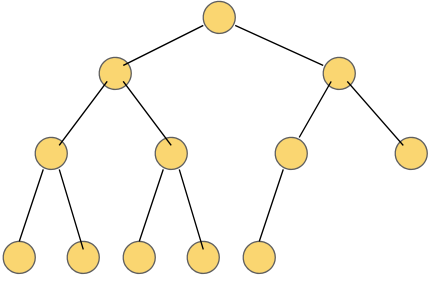
\includegraphics[width=10cm]{imagens/arvquasecompleta.png}
    \label{cable}
    \caption{Cable 1}
\end{figure}

\newpage

\subsection{Árvore completa}

É uma árvore em que todas as folhas estão no nível d (último nível). Essa é uma árvore "cheia".

Possui 2\^(h-1) nós; De uma maneira mais simples, todos os nós que são

\begin{figure}[h]
    \center
    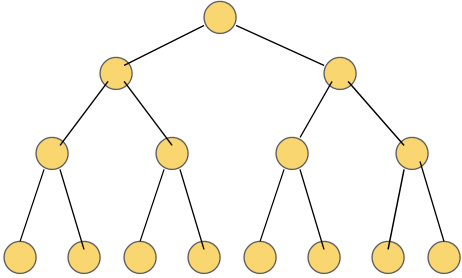
\includegraphics[width=10cm]{imagens/arvcompleta.png}
    \label{cable}
    \caption{Cable 1}
\end{figure}



\subsection{Árvores binárias: Inserção}

Quando você insere o primeiro elemento, ele passa a ser a raíz da nova árvore binária; Na próxima
inserção, ela verifica se existe uma raíz e se ela existe, verifica se esse novo
elemento é maior ou menor que a raíz. Se for maior, você sobe um nível à
esquerda da raíz, ou, se menor, sobe um nível à direita da raiz.\\
Será muito mais fácil entender isso inserindo a seguinte sequência no link de
referência para estudo. Insira, no applet citado, a sequência abaixo e procure
entender como funciona na prática.\\
50, 65, 63, 45, 47, 71, 55 e 46

\subsection{Árvores binárias: Remoção}

O mais importante aqui é manter um padrão de remoção; Escolha um deles e use
sempre o mesmo; Você, quando remover um nó qualquer, X por exemplo, você deve substituí-lo pelo nó de maior nível e mais a esquerda do filho direito de X. Ou você pode escolher o nó direito de maior nível e mais a esquerda do filho esquerdo de X. Se o nó X não tem filhos, não faça nada.\\
Difícil de entender? Olhe os desenhos dos links de referência para estudo. :)

\newpage

\section{Árvores AVL}
O grande problema das árvores binárias de busca é que, embora elas sejam
estruturas mais eficientes que listas, no pior caso elas podem virar uma lista;
Suas alturas também costumam ser grandes, com pouco aproveitamento dos diversos
níveis que ela pode ter.\\Dica: Insira, em uma árvore binária de busca, a
seguinte sequência: 1, 2, 3, 4 e 5. Você terá uma árvore no formato de lista, o
que é ineficiente; A grande sacada das árvores AVL é prover uma técnica que faça
o balanceamento da árvore binária de busca, aproveitando melhor sua estrutura.

\subsection{Links de referência para estudo}
\begin{itemize}
	\item \href{http://equipe.nce.ufrj.br/adriano/c/apostila/arvore.htm}{Árvores AVL: o básico}
	\item \href{http://www.dei.isep.ipp.pt/~hleitao/EI/ARVORESAVL.pdf}{Árvores AVL: Inserção, remoção etc}
	\item \href{http://www.icmc.usp.br/~sce182/arvbinrb.html}{Árvores AVL: Rebalanceamento}
	\item \href{http://www.site.uottawa.ca/~stan/csi2514/applets/avl/BT.html}{Inserção na AVL, applet Java}
	\item \href{http://www.lcad.icmc.usp.br/~nonato/ED/AVL/remocao.html}{Remoção na AVL}
\end{itemize}

\subsection{Inserção e remoção}

Igual as árvores binárias de busca. Só deve-se tomar cuidado com o balanceamento dos nós.

\subsection{Rebalanceamento}
Após inserirmos ou removermos um nó, poderemos desbalancear a árvore AVL. Aqui
entra a ideia do Fator de Balanceamento (FB); Não pretendo explicá-lo com
detalhes (leia os links de referência), mas você deve saber cálculá-lo, e bem.\\
Exemplo de cálculo: Escolha um nó qualquer (X, por exemplo) e verifique quantos
nós ele tem a partir do seu filho direito até a folha, no maior caminho possível
até essa folha. Faça a mesma coisa com o filho esquerdo. Agora subtraia-os.
Pronto, o valor obtido é o valor do FB.\\
IMPORTANTE: Sempre assuma uma regra de subtração e continue com ela para sempre,
desde que exercício não diga o contrário; Por exemplo: Escolho sempre
subtrair a quantidade de nós do filho direito da quantidade de nós do filho esquerdo.
Sempre fazendo da mesma maneira, não tem erro.\\
A árvore está desbalanceada sempre que você encontrar um |FB| > 1; O FB pode ser
qualquer valor dentro do conjunto dos inteiros, mas acima de 1, do módulo de FB,
indica um desbalanceamento. Exemplos: FB=-2, FB=2, FB=3 etc indicam uma árvore
desbalanceada. FB=1, FB=-1 e FB=0 não indicam desbalanceamento.\\
Rotações serão necessárias para corrigir o desbalanceamento, uma para cada caso;
Os links de referência explicam muito bem, então deixo essa responsabilidade a
eles, contudo é MUITO IMPORTANTE que nunca você continue inserindo se a árvore
ficar desbalanceada. Se ela ficar faça o rebalanceamento e SOMENTE DEPOIS DE BALANCEADA continue inserindo ou removendo.

\section{Árvore B}

Links usados como referência:

\begin{itemize}
   \item \href{http://www.lcad.icmc.usp.br/~nonato/ED/B\_arvore/btree.htm}{http://www.lcad.icmc.usp.br/~nonato/ED/B\_arvore/btree.htm}
\end{itemize}

Usada para indexar páginas em um disco rígido. A memória principal é dividida em "molduras de
páginas" e cada moldura contém exatamente uma página.\\

Algumas características da Árvore B:

\begin{itemize}
   \item Generalização da árvore 2-3-4;
   \item Todos os caminhos da raíz a folha tem o mesmo comprimento;
   \item Os blocos de chaves são organizados para estarem pelo menos meio cheios até cheios;
   \item Um bloco tem n chaves e n+1 ponteiros;
   \item Existe um número máximo e mínimo de filhos em um nó. Este número pode ser descrito em
termos de um inteiro fixo t maior ou igual a 2 chamado grau mínimo; 
   \item Todo o nó diferente da raiz deve possuir pelo menos t-1 chaves. Todo o nó interno diferente
da raiz deve possuir pelo menos t filhos. Se a árvore não é vazia, então a raiz possui pelo menos
uma chave;
   \item Todo o nó pode conter no máximo 2t - 1 chaves. Logo um nó interno pode ter no máximo 2t
filhos. Dizemos que um nó é cheio se ele contém 2t - 1 chaves;
   \item A árvore B mais simples ocorre quando t=2. Neste caso todo o nó diferente da raíz possui 2,
3 ou 4 filhos. Esta árvore também é conhecida por árvore 2-3-4.
   \item A altura máxima de um nó  é log\_t((n+1)/2);
   \item Dizemos que uma árvore B é de ordem n quando n representa o número máximo de filhos de um
nó, exceto a raiz. Por exemplo, uma árvore B de ordem 4 pode conter no máximo oito e no mínimo
quatro filhos em cada nó. Porém a palavra "ordem" é usada de formas diferentes pelos autores,
podendo indicar o número máximo de chaves em cada nó, ou até mesmo a ocupação mínima em cada nó.
\end{itemize}

\newpage

Exemplo de um nodo de grau t=2:

\begin{figure}[h]
    \center
    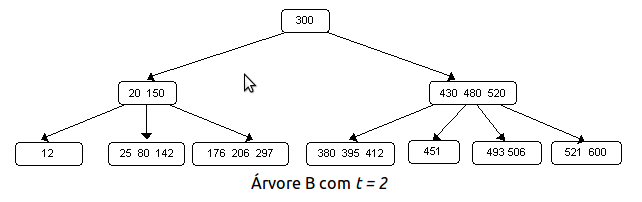
\includegraphics[width=10cm]{imagens/arvb2.png}
    \label{cable}
    \caption{Cable 1}
\end{figure}

Exemplo de um nodo:

\begin{figure}[h]
    \center
    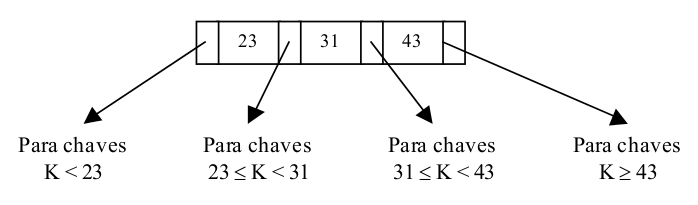
\includegraphics[width=10cm]{imagens/arvb1.png}
    \label{cable}
    \caption{Cable 1}
\end{figure}

\newpage

\subsection{Busca em Árvore B}

A busca em uma árvore B é uma função parecida com a de busca em uma árvore de busca binária, exceto
o fato de que se deve decidir entre vários caminhos. Como as chaves estão ordenadas, basta realizar
uma busca binária nos elementos de cada nó. Isso levará tempo O(lg(t)). Se a chave não for
encontrada no nó em questão, continua-se a busca nos filhos deste nó, realizando-se novamente a
busca binária. Caso o nó não esteja contido na árvore a busca terminará ao encontrar um ponteiro
igual a NULL, ou de forma equivalente, verificando-se que o nó é uma folha. A busca completa pode
ser realizada em tempo O(lg(t)logt(n)).

\subsection{Inserção em Árvore B}

Para inserir um novo elemento em uma árvore B, basta localizar o nó folha X onde o novo elemento
deva ser inserido. Se o nó X estiver cheio, será necessário realizar uma subdivisão de nós que
consiste em passar o elemento mediano de X para seu pai e subdividir X em dois novos nós com t - 1
elementos e depois inserir a nova chave.

\begin{figure}[h]
    \center
    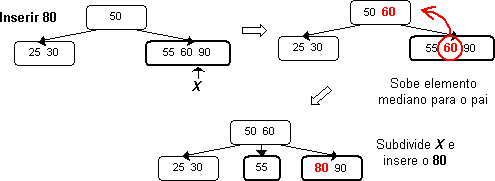
\includegraphics[width=10cm]{imagens/arvb3.png}
    \label{cable}
    \caption{Cable 1}
\end{figure}

Se o pai de X também estiver cheio, repete-se recursivamente a subdivisão acima para o pai de X. No
pior caso terá que aumentar a altura da árvore B para poder inserir o novo elemento.
Note que diferentemente das árvores binárias, as árvores B crescem para cima. A figura abaixo
ilustra a inclusão de novos elementos em uma árvore B com t=3.

\begin{figure}[h]
    \center
    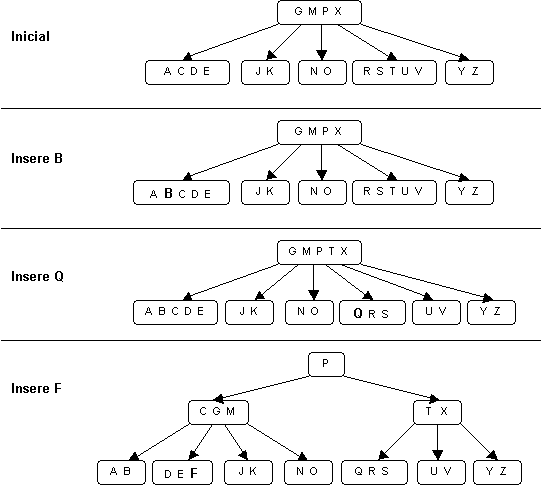
\includegraphics[width=10cm]{imagens/arvb4.png}
    \label{cable}
    \caption{Cable 1}
\end{figure}

\newpage

Mais um exemplo de inserção:
\begin{figure}[h]
    \center
    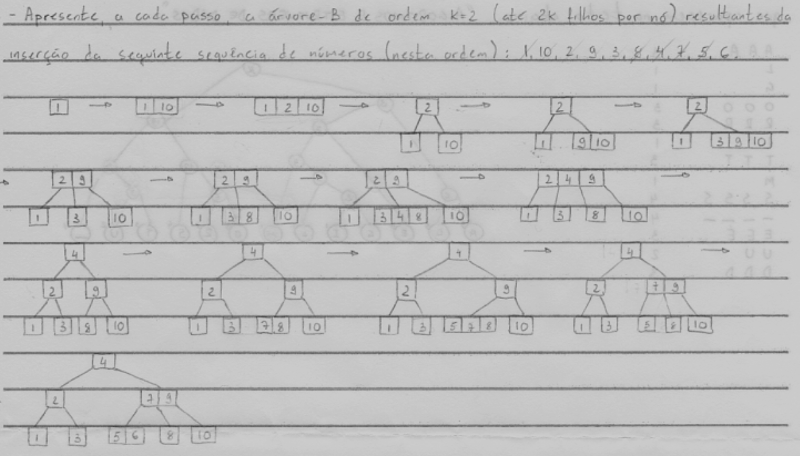
\includegraphics[width=10cm]{imagens/arvb8.png}
    \label{cable}
    \caption{Cable 1}
\end{figure}

\newpage

\subsection{Remoção em Árvore B}

A remoção de um elemento de uma árvore B pode ser dividida em dois casos:

\begin{enumerate}
   \item O elemento que será removido está em uma folha;
   \item O elemento que será removido está em um nó interno;
\end{enumerate}

Se o elemento estiver sendo removido de um nó não folha, seu sucessor, que deve estar em uma
folha, será movido para a posição eliminada e o processo de eliminação procede como se o elemento
sucessor fosse removido do nó folha.\\
Quando um elemento for removido de uma folha X e o número de elementos no nó folha diminui para
menos que t - 1, deve-se reorganizar a árvore B. A solução mais simples é analisarmos os irmãos da
direita ou esquerda de X. Se um dos irmãos (da direita ou esquerda) de X possui mais de t - 1
elementos, a chave k do pai que separa os irmãos pode ser incluída no nó X e a última ou primeira
chave do irmão (última se o irmão for da esquerda e primeira se o irmão for da direita) pode ser
inserida no pai no lugar de k.

\begin{figure}[h]
    \center
    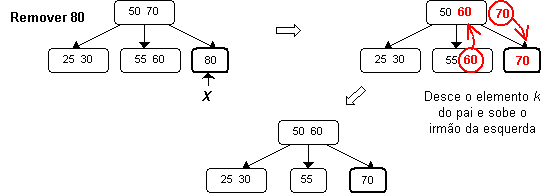
\includegraphics[width=10cm]{imagens/arvb5.png}
    \label{cable}
    \caption{Cable 1}
\end{figure}

Se os dois irmãos de X contiverem exatamente t - 1 elementos (ocupação mínima), nenhum elemento
poderá ser emprestado. Neste caso, o nó X e um de seus irmãos são concatenados em um único nó que
também contém a chave separadora do pai.

\begin{figure}[h]
    \center
    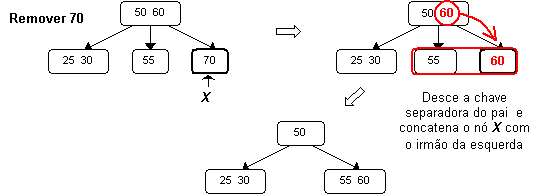
\includegraphics[width=10cm]{imagens/arvb6.png}
    \label{cable}
    \caption{Cable 1}
\end{figure}

Se o pai também contiver apenas t - 1 elementos, deve-se considerar os irmãos do pai como no caso
anterior e proceder recursivamente. No pior caso, quando todos os ancestrais de um nó e seus irmãos
contiverem exatamente t - 1 elementos, uma chave será tomada da raiz e no caso da raiz possuir
apenas um elemento a árvore B sofrerá uma redução de altura.

A figura abaixo ilustra a remoção de elementos em uma árvore B com t=3.

\begin{figure}[h]
    \center
    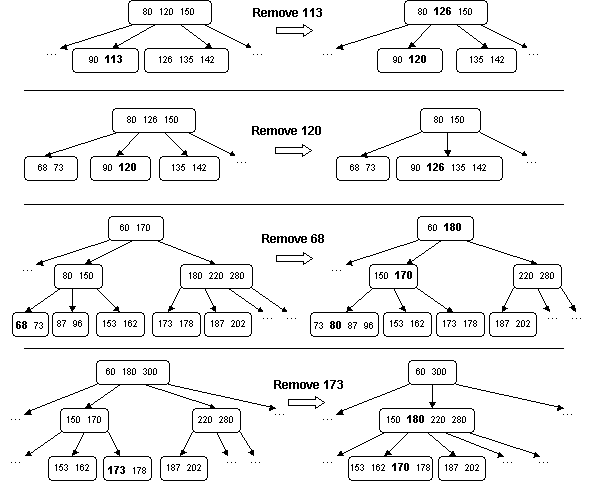
\includegraphics[width=10cm]{imagens/arvb7.png}
    \label{cable}
    \caption{Cable 1}
\end{figure}

\newpage

\section{Árvore Trie:}

Vatangens sobre as árvores binárias:

\begin{itemize}
   \item A busca é mais rápida;
   \item Árvore Trie requer menos espaço quando contém um grande número de cadeias curtas, porque as chaves
não são armazenadas de forma explícita e os nodos das chaves iniciais comuns são compartilhados.
\end{itemize}

Informações importantes sobre a árvore Trie:

\begin{itemize}
   \item Similar as árvores de busca digitais, mas mantém as chaves em ordem e armazena chaves
somente nas folhas;
   \item Definição: Uma trie é uma árvore binária que possui chaves associadas aos nodos folhas e definida recursivamente da seguinte forma:
      \begin{enumerate}
         \item A trie para um conjunto vazio de chaves é apenas um apontador NULL;
         \item A trie para apenas uma chave é composta apenas por um nodo folha que contém esta
chave;
         \item A trie para um conjunto de chaves maior que um é composta por um nodo interno, sendo
o filho esquerdo uma trie contendo chaves  cujo bit inicial é 0 e o filho direito uma trie contendo
chaves cujo bit inicial é 1. O primeiro bit é então removido para a construção das subarvores direita e esquerda.
         \item Se isso tudo não ficou muito claro, fique tranquilo e continue lendo essa
apostila...
      \end{enumerate}
\end{itemize}

Algumas características das árvores Tries:

\begin{itemize}
   \item Chaves só nas folhas;
   \item Mantém árvore em ordem;
   \item Independe da ordem de inserção: Uma única Trie para determinadas chaves.
\end{itemize}

As Tries são boas para suportar tarefas de tratamento
lexicográfico, tais como:

\begin{itemize}
   \item Manuseamento de dicionários;
   \item Pesquisas em textos de grande dimensão;
   \item Construção de índices de documentos;
   \item Expressões regulares (padrões de pesquisa).
\end{itemize}

Cada chave é codificado por uma certa quantidade de bits. Por exemplo:\\
A 00001\\
S 10011\\
E 00101\\
R 10010\\
C 00011\\
H 01000\\
I 01001\\
N 01110\\
G 00111\\
X 11000\\
M 01101\\
P 10000\\
L 01100\\

A inserção se dá justamente analisando esses bits.\\
Se quisessemos inserir A, a raíz seria a novo com a chave A. Ao inserirmos S, devemos localizar qual
bit diferencia A de S. Nesse caso, teríamos:

\begin{figure}[h]
    \center
    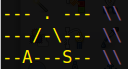
\includegraphics[width=10cm]{imagens/trie1.png}
    \label{cable}
    \caption{Cable 1}
\end{figure}

Observe que A foi para a esquerda, pois o bit que o diferencia de S é o bit zero. Como o bit zero de
A é zero, ele vai para a esquerda. Como o bit zero de S é 1, ele vai para a direita.\\
Agora se inseríssemos E, observe que ele só se diferencia de A no bit número 2, então teríamos:

\begin{figure}[h]
    \center
    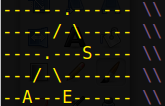
\includegraphics[width=10cm]{imagens/trie2.png}
    \label{cable}
    \caption{Cable 1}
\end{figure}

Observe que E vai para a direita porque seu bit dois é 1 e A para a esquerda porque seu bit dois é
0. E assim por diante nós construímos uma árvore Trie.\\
\textbf{Problema das árvores Tries:} Requer a criação de múltiplos nodos
quando as chaves diferem apenas nos bits no final da chave. Solução: Árvore Patrícia.

\newpage

\section{Trie n-aria:}
Generalizacao de tries, na qual chaves sao codificadas em uma base qualquer,
não necessariamente binária.\\

Uma trie n-aria possui chaves armazenadas nas folhas.  Ela é definida da seguinte forma: uma trie
para um conjunto vazio de chaves corresponde ao apontador nulo; Uma trie com uma única chave corresponde a uma folha contendo 
esta chave; Uma trie com cardinalidade maior que um é um nodo interno com apontadores referentes a
trie com chaves começando com cada um dos digitos possíveis, com este digito desconsiderado na
construção das subarvores.\\

Exemplo: Números na base decimal com 5 digitos\\

\begin{figure}[h]
    \center
    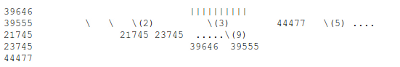
\includegraphics[width=10cm]{imagens/trienaria.png}
    \label{cable}
    \caption{Cable 1}
\end{figure}


\section{Trie existencial:}
Não guarda informação sobre o registro, apenas se uma determinada chave está presente ou não na trie
(n-aria).\\
Uma trie existencial para um conjunto de chaves é definida da seguinte forma: uma trie para um
conjunto vazio de chaves corresponde ao apontador nulo; Uma trie para um conjunto não vazio de
chaves corresponde a um nodo interno com apontadores para nodos filhos contendo valores para cada
valor de dígito possível. Nestas subárvores o primeiro digito é removido para sua construção, de forma recursiva.

\section{Trie Ternária}
Similar as árvores de busca binárias, mas que utiliza caracteres (dígitos) como chave do nodo.
\\Cada nodo tem 3 apontadores: para chaves que comecam com o digito menor que o corrente, iguais e
maiores.\\

Características:

\begin{itemize}
   \item Tempo de busca: tamanho da chave;
   \item Número de links: no máximo 3 vezes o tamanho total do conjunto de chaves.
\end{itemize}

Vantagens da árvore:

\begin{itemize}
   \item Adapta-se as irregularidades (desbalanceamento dos caracteres que parecem) nas chaves de
pesquisa;
   \item Não dependem da quantidade de digitos (caracteres) possíveis;
   \item Quando a chave não está armazenada na árvore, a quantidade de dígitos comparados tende a ser pequena (mesmo quando a chave de busca
é longa);
   \item Ela é flexível:
      \begin{itemize}
         \item Pode ser usada para obter chaves que casam com digitos especificos da chave
de pesquisa;
         \item Pode ser usada para obter chaves que diferem em no máximo uma posição da chave de
pesquisa;
         \item Árvore Patrícia oferece vantagens similares, mas comparando bits ao inves de bytes.
      \end{itemize}
\end{itemize}

Uma vantagem em relação a árvore existencial: Sem dependências em relação ao alfabeto.\\
Um problema: De acordo com a forma da inserção, ela poderá ter um forte desbalanceamento.

\newpage

\subsection{Inserção na ternária:}

Inserindo a palavra CASA:\\
\begin{figure}[h]
    \center
    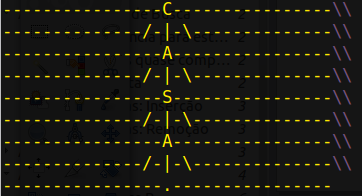
\includegraphics[width=10cm]{imagens/ternaria1.png}
    \label{cable}
    \caption{Cable 1}
\end{figure}

Apenas para a primeira palavra denotarei os ponteiros: esquerda, meio e direita. Esquerdo para quando
a chave for menor, meio para quando a chave casou com a chave do nodo, e direita para quando for
maior.\\

Agora a palavra BELA:\\
\begin{figure}[h]
    \center
    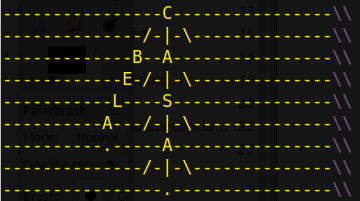
\includegraphics[width=10cm]{imagens/ternaria2.png}
    \label{cable}
    \caption{Cable 1}
\end{figure}

Agora a palavra CARA:\\
\begin{figure}[h]
    \center
    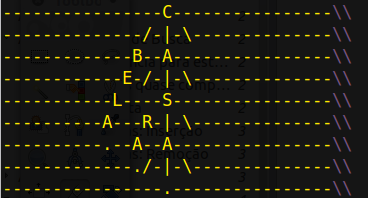
\includegraphics[width=10cm]{imagens/ternaria3.png}
    \label{cable}
    \caption{Cable 1}
\end{figure}

Observe que ele andou por: C, A e quando chegou em S, como R é menor que S, vai a esquerda de S.\\

Agora a palavra RUA:\\
\begin{figure}[h]
    \center
    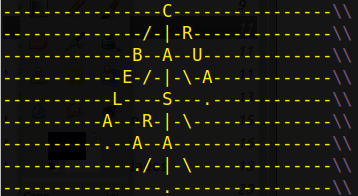
\includegraphics[width=10cm]{imagens/ternaria4.png}
    \label{cable}
    \caption{Cable 1}
\end{figure}

Agora a palavra CASAMENTO:\\
\begin{figure}[h]
    \center
    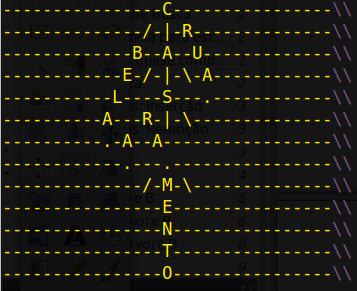
\includegraphics[width=10cm]{imagens/ternaria5.png}
    \label{cable}
    \caption{Cable 1}
\end{figure}

Note que para separar duas palavras diferentes (CASA e CASAMENTO), haverá um nodo "." sempre ao
final de cada palara.\\Infelizmente antes do ponto que separa "MENTO" de "CASA" o A ficou um
pouquinho a esquerda, apenas um erro gráfico. Ele deveria estar abaixo de S.

Melhoramentos possíveis para essa árvore:

\begin{enumerate}
   \item Como a maioria dos nodos proximos das folhas possuem apenas um único filho, utilizar a
mesma ideia das árvores trie n-arias de manter a chave na folha no nível que a distingue das demais
chaves. Isso tornará a árvore *independente* do tamanho das chaves;
   \item Utilizar a ideia das árvore Patricia de manter as chaves nos nodos internos, usando os
apontadores "para cima";
   \item Usar um vetor com N elementos, um para cada dígito possível somente na raiz (busca similar
a um catálogo telefônico).  O objetivo é diminuir a altura da árvore e o número de comparações em uma busca.
\end{enumerate}

\newpage

\section{Heap}

Existem dois tipos de heaps:
\begin{enumerate}
   \item Os heaps de máximo (max heap), em que o valor de todos os nós são
menores que os de seus respectivos pais;
   \item E os heaps de mínimo (min heap), em que o valor todos os nós são maiores que os de seus respectivos pais.
\end{enumerate}

Assim, em um heap de máximo, o maior valor do conjunto está na raíz da árvore, enquanto no heap de
mínimo a raíz armazena o menor valor existente.\\

A árvore binária do heap deve estar completa até pelo menos seu penúltimo nível e, se o seu último
nível não estiver completo, todos os nós do último nível deverão estar agrupados à esquerda.\\

\newpage

Exemplo de uma Heap sort máximo a partir de um vetor desordenado:\\

Primeiro inserimos o vetor na Heap (esquerda para a direita, de cima para baixo).\\
Depois passamos a identificar os problemas. Na heap maxima, todos os filhos devem ser menor que seus
pais, e não maiores.\\

Veja que 16 é maior que 1 e além disso 14 e 8 são maiores que 2:

\begin{figure}[h]
    \center
    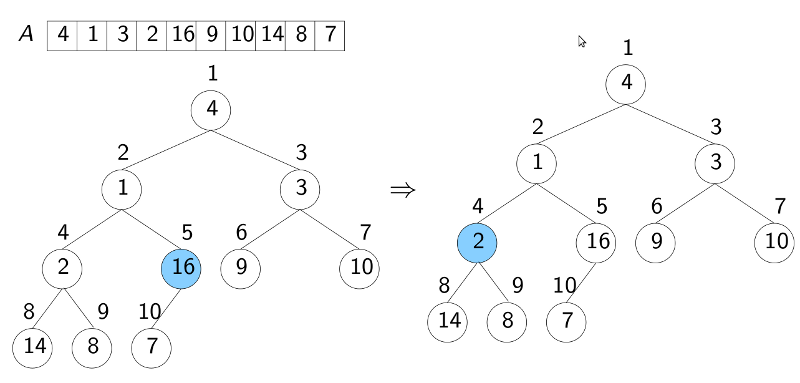
\includegraphics[width=10cm]{imagens/heap1.png}
    \label{cable}
    \caption{Cable 1}
\end{figure}

Note ainda que 3 é menor que 9 e 10. Permutamos 14 e 2 para resolver o problema anterior (vamos
resolvendo de baixo pra cima). Permutamos sempre o filho maior com o nodo pai (por isso escolhemos
14 e não 8).

\begin{figure}[h]
    \center
    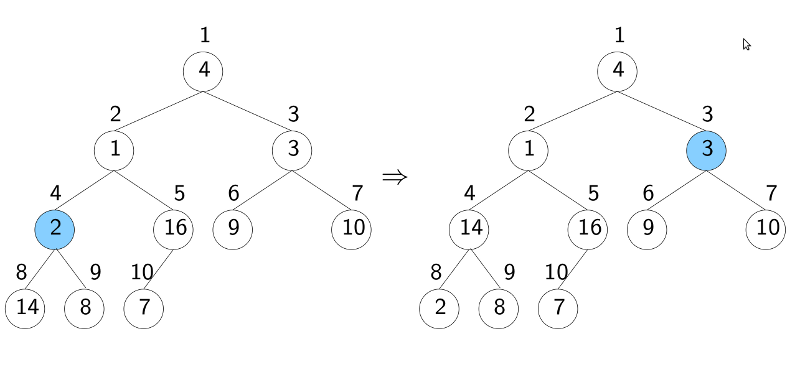
\includegraphics[width=10cm]{imagens/heap2.png}
    \label{cable}
    \caption{Cable 1}
\end{figure}

Subimos o 10 no lugar do 3. Pronto, essa subárvore ficou arrumada.

\begin{figure}[h]
    \center
    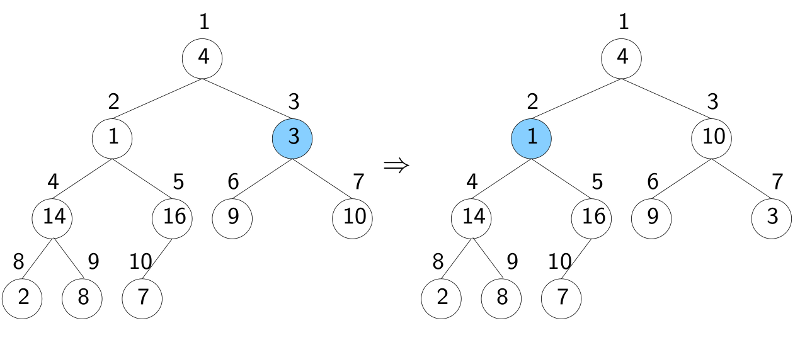
\includegraphics[width=10cm]{imagens/heap3.png}
    \label{cable}
    \caption{Cable 1}
\end{figure}

\newpage

Agora subimos 16, para que ele seja pai de 14 e 1. Como 1 será menor que 7, já aproveitamos e
baixamos 1 e subimos 7. Observe agora que 4 é maior que seus dois filhos. Então subimos 16 para o
lugar de 4 e 14 para o seu lugar. Mas onde irá parar 4? Como 14 subiu para o local anterior de 16, 8
ficará no local anterior de 14 e, portanto, 4 tomará o local anterior de 8. Pronto, a max heap está
pronta.

\begin{figure}[h]
    \center
    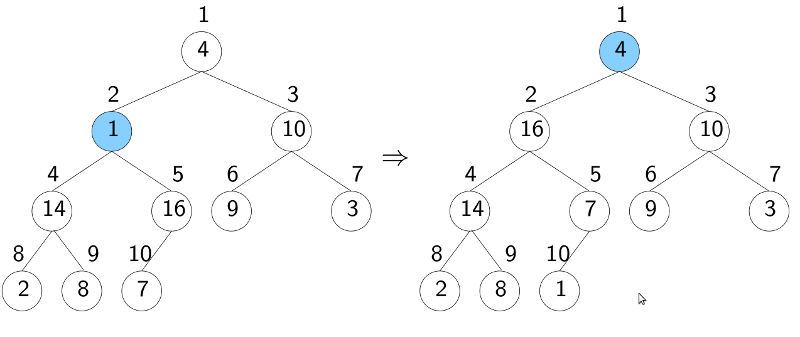
\includegraphics[width=10cm]{imagens/heap4.png}
    \label{cable}
    \caption{Cable 1}
\end{figure}

\begin{figure}[h]
    \center
    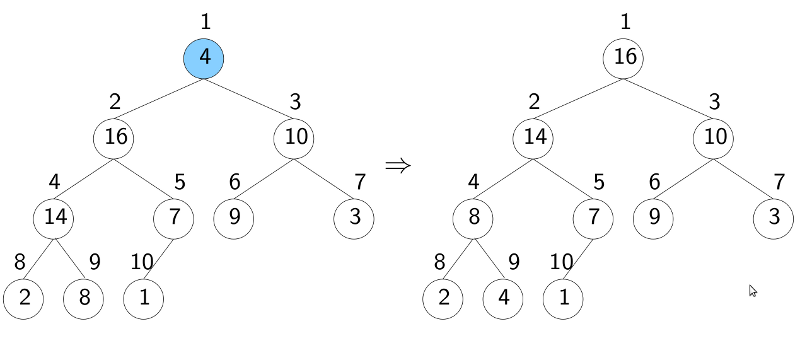
\includegraphics[width=10cm]{imagens/heap5.png}
    \label{cable}
    \caption{Cable 1}
\end{figure}

Embora o custo do heapsort seja o mesmo do quicksort, na prática o quicksort em geral é mais rápido.
Mas uma das aplicações para o heap é a implementação de uma lista de prioridades.\\

Que tal agora construir um vetor na ordem decrescente? Vá removendo as raízes! Por exemplo: Remova o
16 e guarde em v[0]. Arrume a heap. Guarde 14 em v[1]. Arrume a heap. E assim até que a heap não
mais tenha nodos.\\

E como inserir na heap? Insira como se fosse uma árvore binária. Depois vá arrumando de acordo com
sua heap (max ou min) de baixo para cima.

\newpage

\section{Ordenação externa}

Necessária quando a quantidade a ser ordenada não cabe na memória principal.\\

Algumas considerações:
\begin{itemize}
   \item O custo para acessar um item é algumas ordens de grandeza maior que o os custos de
processamento na memória interna. Assim, o custo de um algoritmo de ordenação externa considera
apenas a quantidade de leituras e escritas em memória secundaria, ignorando o custo de processamento
em memória principal;
   \item Podem existir restrições quanto ao acesso aos dados (sequencial/randômico);
   \item O desenvolvimento de algoritmos é muito dependente do estado atual da tecnologia.
\end{itemize}

Estratégia principal para ordenação: 2 passos:

\begin{enumerate}
   \item A primeira passada sobre o arquivo quebrando em blocos do tamanho da
memória interna disponível. Cada bloco é ordenado na memória interna;
   \item Os blocos ordenados são intercalados, fazendo várias passadas sobre o arquivo até que ele esteja completamente ordenado.
\end{enumerate}

Entrada:

\begin{itemize}
   \item N registros para serem ordenados;
   \item Espaço em memória principal para armazenar M registros;
   \item 2P dispositivos externos.
\end{itemize}

\subsection{Intercalação balanceada de vários caminhos}
Exemplo: INTERCALACAOBALANCEADA  (n=22)\\

Considerando M=3 (3 registros) e P=3 (intercalação de 3 caminhos).\\

\textbf{Etapa 1:} O arquivo é lido do dispositivo 0 de 3 em 3 (M) registros e armazenados em blocos de 3 nos
dispositivos P a 2P-1\\
Resultado: N/M blocos de M registros ordenados (22/3)\\

\textbf{Etapa 2:} Intercalação dos blocos ordenados, escrevendo o resultado nos dispositivos 0 a
P-1, repetindo até que todos os registros estejam ordenados.\\

\textbf{Número de passos:} 1 + log\_{P} (N/M)
Exemplo: N (numero de registros) =1.000.000.000, M (espaco para M registros)=1.000.000 e P=3 (3
caminhos): Precisa de apenas 9 passos (1+log\_3 (1.000.000.000/1.000.000)

\subsection{Seleção por substituição}

\begin{itemize}
   \item A implementação do método de intercalação balanceada pode ser realizada utilizando filas de
prioridades;
   \item As duas fases do método podem ser implementadas de forma eficiente e elegante;
   \item Operações básicas para formar blocos ordenados: Obter o menor dentre os registros presentes
na memória interna. Substituí-lo pelo próximo registro da fita de entrada;
   \item Estrutura ideal para implementar as operações: heap.
   \item Operação de substituição: Retirar o menor item da fila de prioridades; Colocar um novo item
no seu lugar. Reconstituir a propriedade do heap.
\end{itemize}

Objetivo: Obtenção de sequências maiores que M no primeiro passo utilizando uma lista de
prioridades.\\

Para números randômicos, o tamanho da sequência gerada é, em média, igual a 2M.\\

Exemplo com heap size = 3: O heap pode também ser utilizado para fazer as intercalações, mas só é
vantajoso quando a quantidade de blocos gerados na primeira fase for grande (maior ou igual a 8).  Neste caso,
será necessário log\_2(8) comparações para obter o menor elemento.

\section{Hash}

O que é endereçamento direto? Se eu quero endereçar [0,n] chaves, então alocar um vetor de n+1
posições. Problema: n pode ser muito grande e a minha busca por n provavelmente sairá caro.\\

Motivação da hashing: Através de uma função posso calcular um local para armazenar minha chave em
minha estrutura. Problema: Podem haver colisões de dados (a função f pode gerar dois endereços
iguais para chaves diferentes).\\

A função hash ideal é aquela que é simples de ser computada e oferece a menor quantidade de colisões
possível.

\subsection{Tratamento de colisões}

\textbf{Endereçamento fechado: Lista encadeada:}\\
Dada uma função Hash, se ocorre uma colisão, as chaves são inseridas em uma lista encadeada naquela
posição da estrutura usada. E assim toda colisão para aquela posição, inserirá linearmente a chave
naquela lista encadeada. Obviamente que essa lista poderá inclusive ser maior que a sua própria
estrutura de armazenamento, não sendo a melhor opção para vários casos.\\

\textbf{Endereçamento aberto: Hash linear e duplo.}\\

O Hash Linear consiste em:

\begin{itemize}
   \item Exemplo: h(k,i) = (h'(k) + i) mod m
   \item Dada uma função Hash, ocorre uma colisão;
   \item Se ocorreu uma colisão, o algoritmo irá procurar o próximo endereço livre da sua estrutura
e usá-lo para guardar a chave que colidiu;
   \item Problema: Agrupamento de endereços ocupados. Se numa busca você tiver de procurar essa
chave e não encontrá-la na resposta da sua função Hash, então você terá de fazer uma busca linear a
partir do endereço resultado da sua função Hash;
\end{itemize}

O Hash duplo consiste em:

\begin{itemize}
   \item Exemplo: h(k,i) = (h1(k) + i*h2(k)) mod m
   \item Utiliza-se duas funções de Hash para resolver a colisão;
   \item Se a primeira função Hash colide, utilizamos então a segunda função.
   \item Se a segunda função colide, basta incrementar uma variável (no exemplo, i) que fará um deslocamento simples
computacionalmente e que, se bem feita, poderá garantir que a sequência de endereços dada a uma
chave pela função de hash dupla será diferente de outras chaves que colidiriam já na primeira
função, diminuindo a possibilidade de novas colisões;
   \item Exemplo prático: m=13; h1(k) = k mod 13, h2(k) = 1 + (k mod 11), sendo k uma chave m um
número primo (um primo não próximo da uma potência de dois).

\end{itemize}

\subsection{Funções Hash}

Segue alguns tipos de funções Hash.\\

Método da divisão:

\begin{itemize}
   \item h(k) = k mod m, sendo k a chave e m um número primo não próximo a uma potência de dois.
\end{itemize}

Método da multiplicação:

\begin{itemize}
   \item h(k) = floor(m * (k*A mod 1), sendo m um número primo não próximo a uma potência de dois, k
uma chave e A uma constante que varia entre 0 e 1;
   \item Vantagem: Método não muito dependente de m.
\end{itemize}

Hashing Universal:

\begin{itemize}
   \item Escolha de uma função Hash randomicamente que seja independente do valor da chave;
   \item Algoritmo poderá ter comportantemente distinto em cada execução e nem sempre há como prever
se será uma função Hash bem espalhada em seus resultados ou não.
\end{itemize}

\newpage

\section{Compressão de dados}

Motivação: comprimir dados hehehe...\\

\subsection{Codificação de Huffman}

Ideia de Huffman: Códigos menores são gerados para caracteres que aparecem no texto com maior
frequência. Entenda-se por códigos as representações das palavras em binário.\\

Um preview de uma condificação de Huffman resolvida:

\begin{figure}[h]
    \center
    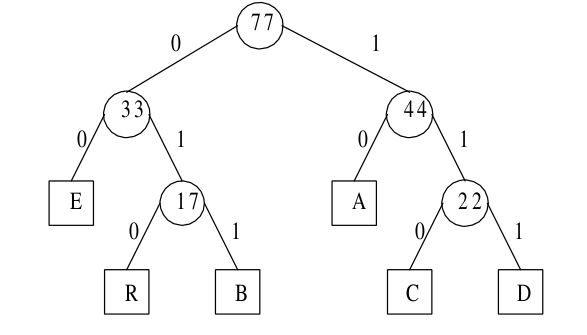
\includegraphics[width=10cm]{imagens/huffman.png}
    \label{cable}
    \caption{Cable 1}
\end{figure}

\newpage

Vou explicar esse preview passo-a-passo de tal maneira que resolver a codificação e a
decodificação seja como tirar doce de criança (ok, nem sempre é tão fácil tirar o doce de um
pivete).\\

Agora devemos pegar nosso texto a ser comprimido e analisar as tuplas (LETRA,FREQUENCIA DAS LETRAS).
Exemplo: (A,22), ou seja, há 22 caracteres "A"). Devemos conhecer quais são as letras mais usadas e as menos usadas. Lembre-se que espaço também é
caracter. O ignorarei aqui.\\

\begin{figure}[h]
    \center
    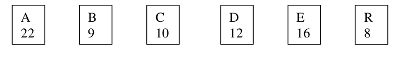
\includegraphics[width=10cm]{imagens/huffman2.png}
    \label{cable}
    \caption{Cable 1}
\end{figure}


Basicamente devemos começar pegando as duas letras com menores frequências e criando uma árvore cujo
único nodo é a raíz, e essa raíz contém a soma das frequências dessas letras.

\begin{figure}[h]
    \center
    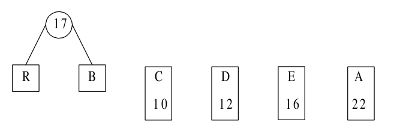
\includegraphics[width=10cm]{imagens/huffman3.png}
    \label{cable}
    \caption{Cable 1}
\end{figure}

\newpage

Para continuar, devemos agora somar os dois outros caracteres com menor frequência.\\
\textbf{Importante:} Se somar o conteúdo de duas raízes, sendo uma delas a de uma árvore já
existente, e for menor que qualquer outra possibilidade de soma, faça sempre a menor soma
possível.\\

\begin{figure}[h]
    \center
    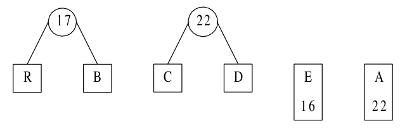
\includegraphics[width=10cm]{imagens/huffman4.png}
    \label{cable}
    \caption{Cable 1}
\end{figure}

\begin{figure}[h]
    \center
    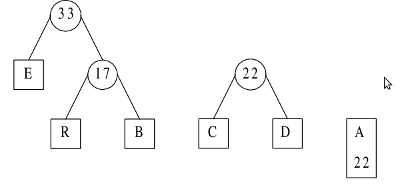
\includegraphics[width=10cm]{imagens/huffman5.png}
    \label{cable}
    \caption{Cable 1}
\end{figure}

\newpage

\begin{figure}[h]
    \center
    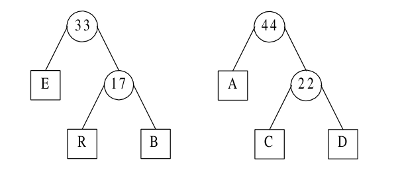
\includegraphics[width=10cm]{imagens/huffman6.png}
    \label{cable}
    \caption{Cable 1}
\end{figure}

Terminamos com duas árvores, agora basta somar as suas raízes e obteremos a árvore de huffman já
previamente apresentada.

\subsection{Decodificação de Huffman}
Suponha que tenhamos recebido a seguinte mensagem:\\
1001101010110101111001101010\\

E conhecemos a codificação dos caracteres:\\
A é representado por 10 (olhe a árvore de Huffman, veja que A está no caminho 10 (uma vez a esquerda
e outra vez a direita).\\
B: 011, C: 110, D: 111, E: 00, R: 010.\\

Você está achando que é loucura decifrar a mensagem? É fácil, muito fácil. Pegue o primeiro bit da
sua mensagem e percorra a árvore de huffman desde a raíz. Quando você cair em uma folha, BAM, você
decodificou um caractere. Parece mágica? Parece impossível? É a árvore de Huffman! :)

\newpage

\section{Árvore B+}

Ideia: separar nodos de indice de nodos de dados

\begin{itemize}
   \item Nodos internos contem apenas índices;
   \item Todos os registros estão nas folhas (sem a necessidade de apontadores);
   \item Os nodos folha são encadeados (para facilitar a busca ordenada de valores);
   \item pode ter um grau distinto para nodos índice e folha.
\end{itemize}

Objetivos:

\begin{itemize}
   \item Acesso sequencial mais eficiente;
   \item Facilitar o acesso concorrente as dados.
\end{itemize}

Acesso concorrente:

\begin{itemize}
   \item Podem ocorrer problemas se um processo estiver lendo a estrutura e outro inserindo uma nova
chave que causa divisão de um nodo;
   \item Uma pagina é segura se não houver possibilidade de mudança na estrutura da árvore devido a
inserção ou remoção na pagina;
   \item Inserção: Página é segura se número de chaves for menor que 2t-1;
   \item Remoção: Página é segura de número de chave for maior que t-1.
\end{itemize}

Protocolo de bloqueio:

\begin{itemize}    
   \item lock-R : bloqueio para leitura;
   \item lock-W: bloqueio exclusivo para escrita.
\end{itemize}

Leitura:

\begin{enumerate}
   \item lock-R(raiz) 
   \item read(raiz)  e torne-a pagina corrente
   \item enquanto página corrente não for folha
   \item lock-R(descendente)
   \item unlock(pag corrente)
   \item read(descendente) e torne-a página corrente
\end{enumerate}

Atualização:

\begin{enumerate}
   \item lock-W(raiz)
   \item read(raiz) e torne-a página corrente
   \item enquanto pag. corrente não for folha
   \item lock-W(descendente)
   \item read(descedente) e torne-a paginal corrente
   \item se página corrente for segura
   \item unlock(p) para todos os nodos p antecedentes que tenham sido bloqueados
\end{enumerate}

\newpage

\section{Método de Acesso Sequencial Indexado (ISAM)}

Caracterísricas:

\begin{itemize}
   \item Parecido com o arvore B+, mas utiliza paginas de overflow;
   \item Há uma previsão inicial da quantidade de registros do arquivo, deixando cerca de 20\% das
paginas inicialmente livres;
   \item vantagem: Não há necessidade de bloqueio nas páginas de índice;
   \item desvantagem:  pode haver um "desequilíbrio" da quantidade de registros em cada intervalo.
\end{itemize}

\newpage

\section{Árvore Patrícia}

Links para estudo:

\begin{itemize}
	\item \href{http://www.ic.unicamp.br/~vanini/mc202/apresentacoes/ArvoreDigital.pdf}{Patrícia e
árvores digitais}
\end{itemize}

\newpage

\section{Árvore Rubro-Negra}

Links para estudo:

\begin{itemize}
	\item \href{http://www.ime.usp.br/~song/mac5710/slides/08rb.pdf}{Rubro-Negra I}
	\item
\href{http://www.ic.unicamp.br/~vanini/mc202/apresentacoes/ArvoresDe\%20BuscaBalanceadas.pdf}{Buscas
balanceadas: avl, rubro-negra etce}
\end{itemize}

Algumas informações importantes:

\begin{itemize}
	\item Ela é complexa, mas apresenta um bom pior-caso e o tempo de execução para as suas operações
é eficiente na prática (busca, inserção e remoção em tempo O(logn));
	\item Usada para implementar vetores associativos;
	\item Tem estrutura similiar a uma árvore 2-3-4 e pode ser permutada para uma árvore 2-3-4. Note
que a arvore 2-3-4 é mais genérica. Podemos a pártir de uma árvore rubro negra ter mais de um tipo
de árvore B;
	\item Altura máxima: 2*log(n+1);
\end{itemize}

\newpage

\subsection{Rubro-negra semelhante a 2-3-4}

Uma árvore rubro-negra tem estrutura similar a uma árvore B de ordem 4, onde cada nó pode conter de 1 até 3 valores e (consequentemente) entre 2 e 4 ponteiros para filhos. Nesta árvore B, cada nó contem apenas um valor associado ao valor de um nó negro da árvore rubro-negra, com um valor
opcional antes e/ou depois dele no mesmo nó. Estes valores opcionais são equivalentes a um nós
vermelhos na árvore rubro-negra.\\

Uma maneira de visualizar esta equivalência é "subir" com os nós vermelhos na representação gráfica
da árvore rubro-negra de modo a alinhá-los horizontalmente com seus pais negros, assim criando uma
lista de nós na horizontal. Tanto na árvore B quanto na representação modificada da árvore
rubro-negra, todos as folhas estão no mesmo nível.\\

Entretanto, esta árvore B é mais geral que uma árvore rubro-negra, já que a árvore B pode ser convertida de mais de uma maneira em uma árvore rubro-negra. Se a lista de valores de um nó da árvore B contém somente 1 valor, então esse valor corresponde a um nó negro com dois filhos. Se a lista contém 3 valores, então o valor central corresponde a um nó negro e os outros dois valores correspondem a filhos vermelhos. Se a lista contém 2 valores, então podemos fazer qualquer um dos valores negro e o outro valor corresponde a seu filho vermelho.

\begin{figure}[h]
    \center
    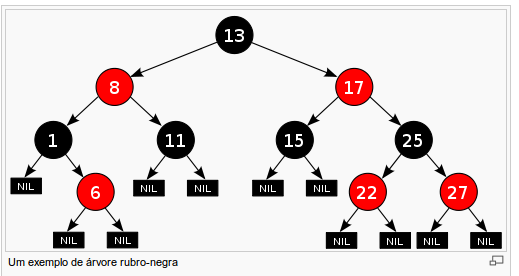
\includegraphics[width=10cm]{imagens/rub1.png}
    \label{cable}
    \caption{Cable 1}
\end{figure}

\begin{figure}[h]
    \center
    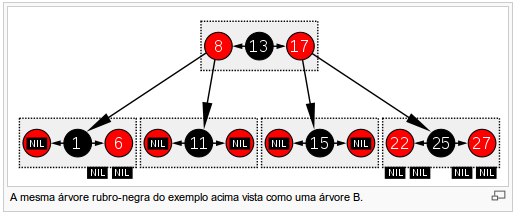
\includegraphics[width=10cm]{imagens/rub2.png}
    \label{cable}
    \caption{Cable 1}
\end{figure}

\newpage

\subsection{}

\end{document}
